\documentclass[
  english,            % define the document language (english, german)
  aspectratio=169,    % define the aspect ratio (169, 43)
  % handout=2on1,       % create handout with multiple slides (2on1, 4on1)
  % partpage=false,     % insert page at beginning of parts (true, false)
  % sectionpage=true,   % insert page at beginning of sections (true, false)
]{tumbeamer}


% load additional packages
\usepackage{booktabs}
\usepackage{amsmath}
\usepackage{amssymb}
\usepackage{mdframed}
\usepackage{amsthm}
\usepackage{mathtools}
\usepackage{multicol}
\usepackage{hyperref}
%\usepackage{julialogo}

\makeatletter
\patchcmd{\@Aboxed}{\boxed{#1#2}}{\fcolorbox{white}{blue!20}{$\displaystyle #1#2$}}{}{}%
\makeatother

\newtheorem{theorem}{Theorem}
\newtheorem{lemma}{Lemma}
\newtheorem{definition}{Definition}
\newtheorem{proposition}{Proposition}
\newtheorem{conjecture}{Conjecture}

%\usepackage{courier}
\usepackage{xcolor}
\usepackage{tikz}
\usepackage{tikzit}
\usetikzlibrary{shapes,arrows,calc,decorations.pathreplacing,angles,quotes}

\input{colors.tikzstyles}

\usepackage{empheq}
\usepackage{tcolorbox}

\tcbset{highlight math style={colback=blue!20!white,arc=2pt,boxrule=0pt}}
\newenvironment{emphbox}
  {\begin{tcolorbox}[colback=blue!5!white,colframe=blue!75!black]}
  {\end{tcolorbox}}


\usepackage{algpseudocodex}
\usepackage{algorithm}

%\colorlet{lightblue}{!10}
\usepackage{listings}
\lstset{
	basicstyle=\ttfamily,
	backgroundcolor = \color{blue!10},
	keywordstyle=\color{blue},
    numberstyle=\tiny\color{codegray},
    stringstyle=\color{purple},
    basicstyle=\ttfamily\footnotesize,
	% numbers=left, 
	numberstyle={\footnotesize \color{blue!50}},
	xleftmargin=.1in,
	numbersep=3pt,
	literate={\$}{{\textcolor{blue}{\$}}}1,
  showlines=true 
}
	
\usepackage{lmodern}

\usepackage{fontawesome}
\usepackage{julialogo}

\usepackage{nameref}
\makeatletter
\newcommand*{\currentname}{\@currentlabelname}
\makeatother
%\usepackage{dsfont}

\newcommand{\R}{{\mathbb R}}
\newcommand{\N}{{\mathbb N}}
\newcommand{\E}{{\mathbb E}}
\renewcommand{\P}{{\mathbb P}}
\newcommand{\bbC}{{\mathbb C}}
\newcommand{\cO}{\mathcal{O}}
\newcommand{\cF}{\mathcal{F}}
\newcommand{\cE}{\mathcal{E}}
\newcommand{\cX}{\mathcal{X}}
\newcommand{\cA}{\mathcal{A}}
\newcommand{\cS}{\mathcal{S}}
\newcommand{\cR}{\mathcal{R}}
\newcommand{\cB}{\mathcal{B}}
\newcommand{\cP}{\mathcal{P}}
\newcommand{\cM}{\mathcal{M}}
\newcommand{\bv}{\mathbf{v}}

\newcommand{\tV}{\widetilde{V}}
\newcommand{\tF}{\widetilde{F}}
\newcommand{\tQ}{\widetilde{Q}}

\newcommand{\bw}{\mathbold{w}}

\newcommand{\step}[1]{\mathds{1}_{\{#1\ge 0\}}}

\newcommand{\eps}{\varepsilon}

\renewcommand{\emph}[1]{\textcolor{purple}{#1}}
\newcommand{\argmax}{\mathop{\textrm{argmax}}}
\newcommand{\mean}{\mathop{\textrm{mean}}}
\newcommand{\diam}{\mathop{\textrm{diam}}}

\DeclareMathOperator*{\esssup}{ess\,sup}


\setbeamertemplate{itemize items}[circle]

% presentation metadata
\title{An introduction to pseudospectra and application to validated computational dynamics}
\author{April Herwig}

\institute{\theChairName\\\theDepartmentName\\\theUniversityName}
\date{}

%\footline{\insertauthor~|~\insertshorttitle~|~\insertshortdate}
\footline{}


% macro to configure the style of the presentation
\TUMbeamersetup{
  title page = TUM centered,         % style of the title page
  part page = TUM toc,            % style of part pages
  section page = TUM toc,         % style of section pages
  content page = TUM more space,  % style of normal content pages
  tower scale = 1.0,              % scaling factor of TUM tower (if used)
  headline = TUM empty,      % which variation of headline to use
  footline = TUM default,         % which variation of footline to use
  % configure on which pages headlines and footlines should be printed
  headline on = {title page},
  footline on = {every page, title page=false},
}

% available frame styles for title page, part page, and section page:
% TUM default, TUM tower, TUM centered,
% TUM blue default, TUM blue tower, TUM blue centered,
% TUM shaded default, TUM shaded tower, TUM shaded centered,
% TUM flags
%
% additional frame styles for part page and section page:
% TUM toc
%
% available frame styles for content pages:
% TUM default, TUM more space
%
% available headline options:
% TUM empty, TUM oneliner, TUM twoliner, TUM threeliner, TUM logothreeliner
%
% available footline options:
% TUM empty, TUM default, TUM infoline

\setlength{\parskip}{1em}

\usepackage{mathpple}
%\usepackage{euler}
%\usepackage{palatino}

\begin{document}

\tikzstyle{block} = [thick, draw, rectangle, rounded corners, fill=blue!20,
                       minimum height=3em, minimum width=6em]
\tikzstyle{node} = [thick, draw, circle, fill=blue!20]
\tikzstyle{action} = [thick, draw, circle, fill=red!10]

\maketitle

\begin{frame}{Contents}
  
\begin{itemize}
  \item Definition (and equivalent formulations) of the $\epsilon$-pseudospectrum $\sigma_\epsilon (M)$
  \item Theoretical results to gain some intuition
  \begin{itemize}
    \item Geometry of $\sigma_\epsilon (M)$
    \item Almost-invariant sets can be obtained from pseudoeigenvalues
  \end{itemize}
  \item A note on backward-stability
  \item How to compute the pseudospectrum
  \begin{itemize}
    \item General inner approximation
    \item Specific methods for Perron-Frobenius / Koopman
  \end{itemize}
\end{itemize}

\end{frame}

\begin{frame}{Pseudospectra}

\begin{definition}

  [Trefethen, Landau, Varah, Godunov, Hinrichsen \& Pritchard]
  The pseudospectrum of a closed linear operator $M : \cX \to \cX$ over a Banach space $\cX$ is the set 
  \begin{equation}
    \sigma_\epsilon (M) = \bigcup_{\| E \|_{op} \leq \epsilon} \sigma (M + E)
  \end{equation}
\end{definition}

\begin{figure}
  \centering
  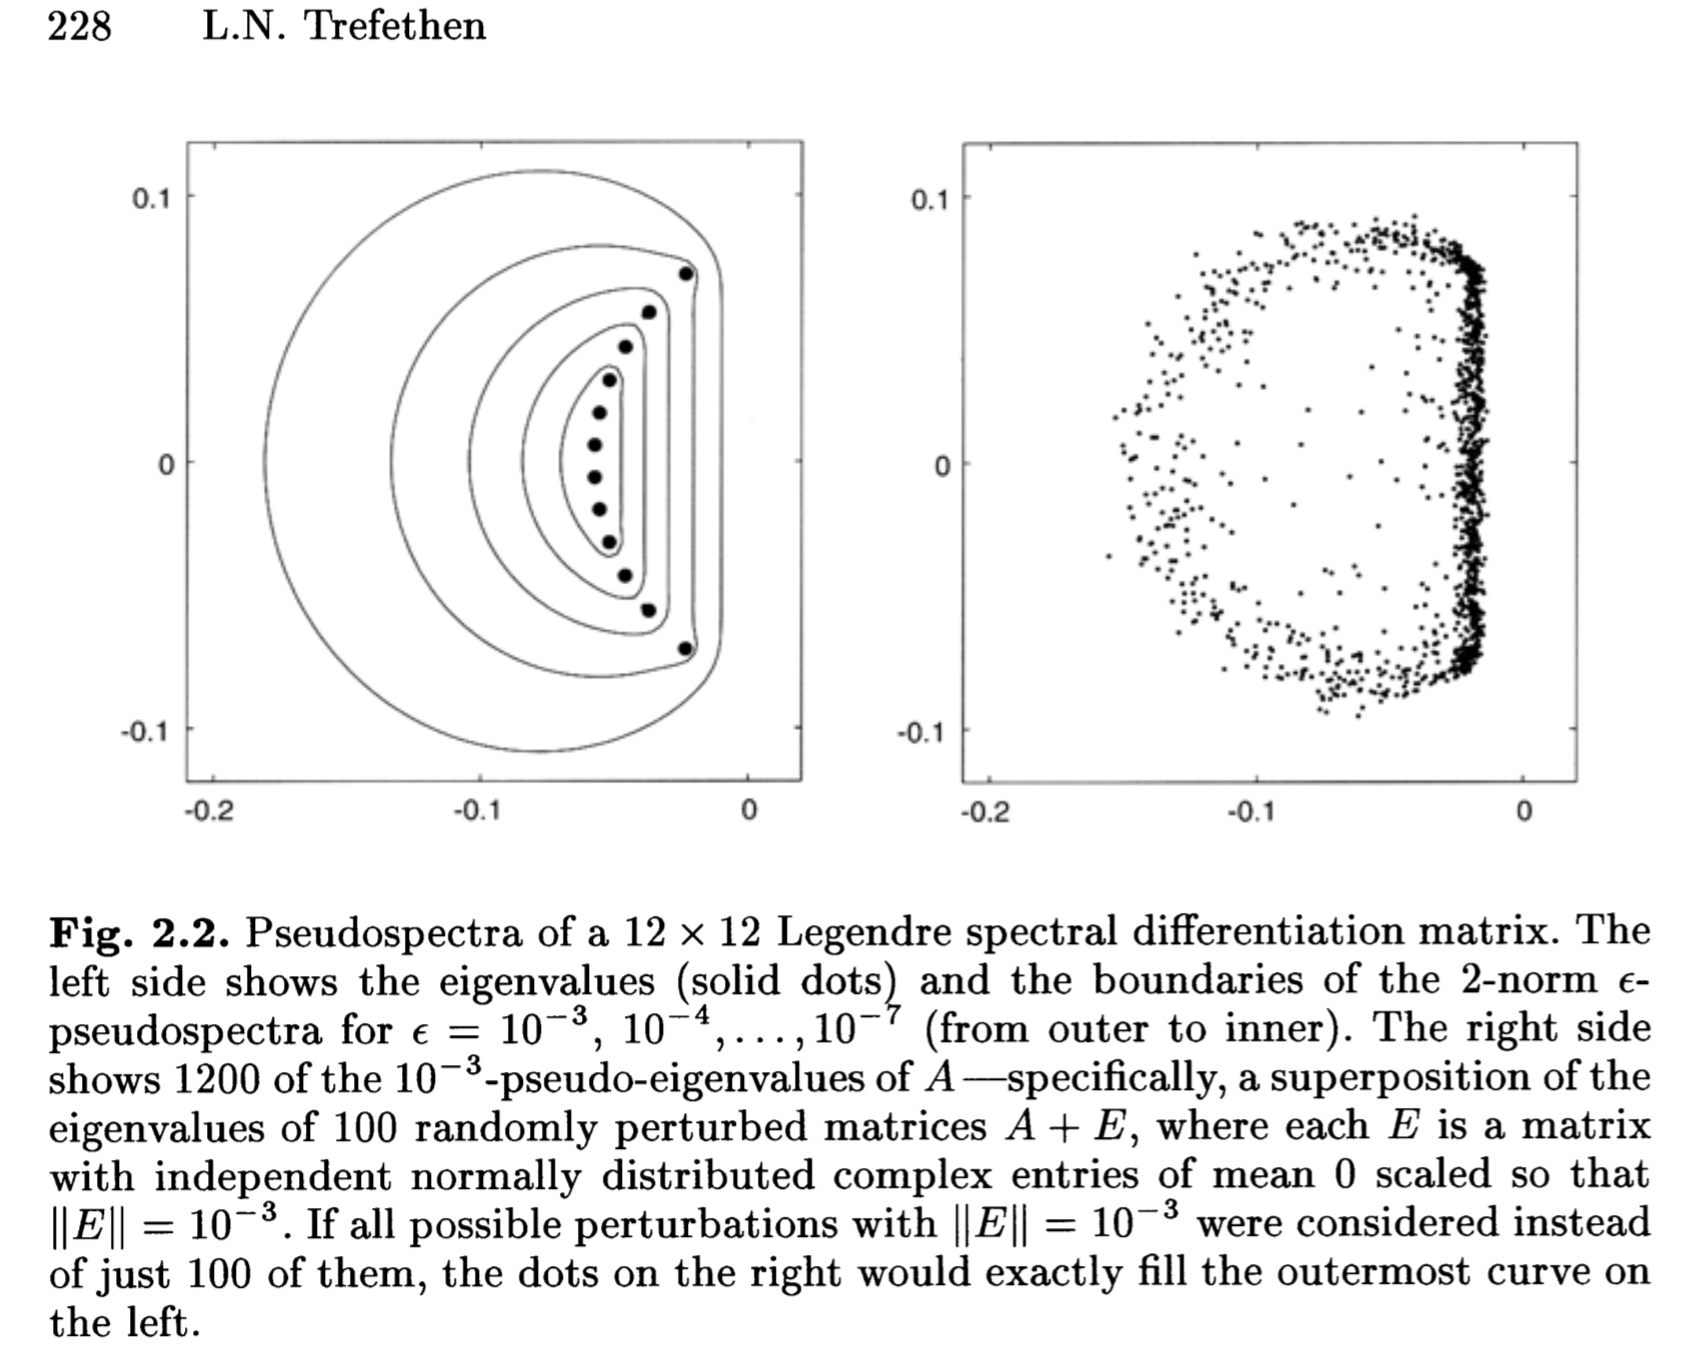
\includegraphics[width=0.4\textwidth]{random_perturbations_of_matrix.jpeg}
\end{figure}

\end{frame}

\begin{frame}{Pseudospectra}
  
\begin{theorem}

  [Trefethen] The following formulations are equivalent:
  \begin{enumerate}[(i)]
    \item \begin{equation}
      \sigma_\epsilon (M) = \bigcup_{\| E \|_{op} \leq \epsilon} \sigma (M + E) \,,
    \end{equation}
    \item \begin{equation}
      \sigma_\epsilon (M) = \left\{ z \in \bbC \mid \| (M - z)^{-1} \|_{op} \geq 1/\epsilon \right\} ,
    \end{equation}
    \item \begin{equation}
      \sigma_\epsilon (M) = \left\{ z \in \bbC \mid \inf_{\| v \| = 1} \| (M - z) v \| \leq \epsilon \right\} ,
    \end{equation}
    \item If $\dim (\cX) < \infty$ is an inner product space, \begin{equation}
      \sigma_\epsilon (M) = \left\{ z \in \bbC \mid s_{min} \leq \epsilon \right\} .
    \end{equation}
  \end{enumerate}
\end{theorem}

\end{frame}

\begin{frame}{Theoretical results}{Geometry of pseudospectra}
  
\begin{theorem} 
  
  [Trefethen]


  \begin{enumerate}[(i)]
    \item If $M$ is normal, $ \sigma_\epsilon (M) =  \sigma (M) + B_\epsilon $ are $\epsilon$-balls around the spectrum.  \vspace*{10ex}
    
    \item $ \bigcap_{\epsilon > 0} \sigma_\epsilon (M) = \sigma (M)\ $ and conversely $\ \sigma_{\epsilon + \delta} (M) \supset \sigma_\epsilon + B_\delta $
  \end{enumerate}
\end{theorem}

\end{frame}

\begin{frame}{Theoretical results}{Almost invariant sets}
  
\begin{theorem}

  [Junge]
\end{theorem}
\begin{figure}
  \centering
  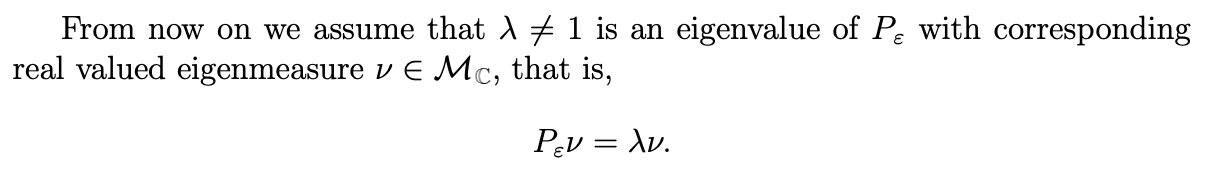
\includegraphics[width=0.5\textwidth]{almost_inv_1.png}
  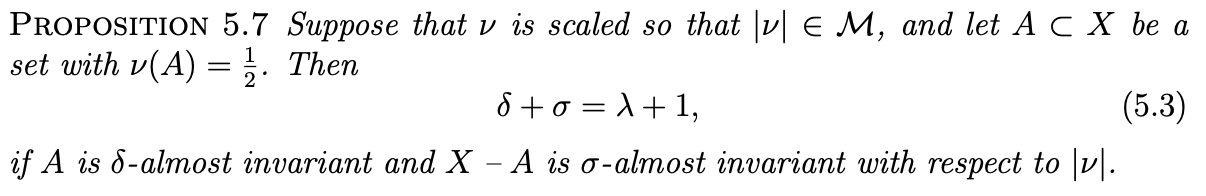
\includegraphics[width=0.5\textwidth]{almost_inv_2.png}
\end{figure}

\begin{theorem}
  Suppose $\nu$ is an $\epsilon$-pseudoeigenmeasure for the pseudoeigenvalue $\lambda \neq 1$ of a Perron-Frobenius operator $P$, where $\epsilon = o (1 - \lambda)$. Suppose further that $\nu$ is scaled so $| \nu | \in \cM$ and $A$ is a set with $\nu (A) = 1/2$. Then 
  \begin{equation}
    \delta + \sigma = 1 + \lambda + o (1 - \lambda)
  \end{equation}
  if $A$ is $\delta$-almost invariant and $X - A$ is $\sigma$-almost invariant with respect to $| \nu |$. 
\end{theorem}

\end{frame}

\begin{frame}{A note on backward-stability}
  
\begin{theorem}
  Let $X$ be a metric space with Borel measure $dx$. Let $S,\hat{S} : X \to X$ be two continuous functions with $ d_{ess}^\infty (S, \hat{S}) > 0 $ \footnote{$\ d_{ess}^\infty (S, \hat{S}) = \esssup_{x}\ d(\, S(x),\, \hat{S}(x)\, )$ refers to the essential supremum distance}. Then the induced Perron-Frobenius (pushforward) operators $P_S, P_{\hat{S}} : \cM \to \cM$ satisfy 
  \begin{equation}
    \| P_S - P_{\hat{S}} \|_{op} \geq 2 . 
  \end{equation}
  This remains true (under adjustment of the const $2$) if $P_S, P_{\hat{S}}$ are induced by (sufficiently) small random perturbations in the sense of [Kifer]. 
\end{theorem}

\begin{emphbox}
  Note that this does \emph{not} contradict the continuous dependence of eigenvalues of $P_S$. 
\end{emphbox}

\end{frame}

\begin{frame}{A note on backward-stability}
  
\begin{proposition}
  \footnote{$\ W_1$ is the Wasserstein-$1$ metric.}
  Let $X$ be a metric space with Borel measure $dx$. Let $S,\hat{S} : X \to X$ be two continuous functions. Then 
  \begin{equation}
    d_{ess}^\infty (S, \hat{S}) < \epsilon 
    \quad \Leftrightarrow \quad 
    W_1 (P_S \varphi, P_{\hat{S}} \varphi) < \epsilon \quad \forall \varphi \geq 0,\, \| \varphi \|_{L^1} = 1 . 
  \end{equation} 
\end{proposition}

\begin{conjecture}
  This remains true (under potential adjustments of constants) if $P_S, P_{\hat{S}}$ are induced by (sufficiently) small random perturbations in the sense of [Kifer]. 
\end{conjecture}

\begin{emphbox}
  This seems to suggest considering a different notion of pseudoeigenvalues
  \begin{equation}
    W_1 ( P_S \varphi, \lambda \varphi ) \leq \epsilon \quad \forall \varphi \geq 0,\, \| \varphi \|_{L^1} = 1 
  \end{equation}
  though this would likely be much more difficult. 
\end{emphbox}

\end{frame}

\begin{frame}{How to compute the pseudospectrum}{General inner approximation}
  
\begin{lemma}
  Let $(V_d)_d$ be a collection of projections which converge pointwise to the identity \footnote{$\ V_d x \xrightarrow{d \to \infty} x \quad \forall x$}. Let 
  \begin{equation}
    (\lambda, x)\ \text{be an}\ \epsilon \text{-pseudoeigenpair for}\ V_d M V_d. 
  \end{equation}
  
  Then $\lambda \in \sigma_{\epsilon + \delta} (M)$ for all $\delta$ and sufficiently large $d = d(\delta, x)$. 
\end{lemma}

\begin{emphbox}
  Note that this does \emph{not} necessarily imply that $\sigma_\epsilon (V_d M V_d) \nearrow \sigma_\epsilon (M)$ as $d \to \infty$.  
\end{emphbox}

\end{frame}

\begin{frame}{How to compute the pseudospectrum}{ResDMD [Colbrook, Townsend]}
  
\begin{itemize}
  \item Given: 
  \begin{itemize}
    \item quadrature scheme $(\, (w^i, x^i) \,)_{i=1}^m$
    \item dictionary $(\, \psi_j \,)_{j=1}^N$ of $L^2$ observables
  \end{itemize}
  \item Data matrices: 
  \begin{align}
    \Psi_X &= \Psi . (\mathbf{x}) = (\psi_1 \ldots \psi_N)\ . 
    \begin{pmatrix}
      x^1 \\
      \vdots \\
      x^m
    \end{pmatrix}
    = \begin{pmatrix}
      \psi_1 (x^1) & \cdots & \psi_N (x^1) \\
      \vdots & & \vdots \\
      \psi_1 (x^m) & \cdots & \psi_N (x^m)
    \end{pmatrix} \\
    \Psi_Y &= (\Psi\ .\circ \,S) . (\mathbf{x})
  \end{align}
  %\begin{equation}
  %  \begin{matrix}
  %    \text{Graham matrix} & & \text{EDMD matrix} & & \text{ResDMD matrix} \\ 
  %    G = \Psi_X ' W \Psi_X &  &A = \Psi_X ' W \Psi_Y & &  L = \Psi_Y ' W \Psi_Y \\ 
  %    \downarrow & \scriptstyle{m \to \infty} & \downarrow & \scriptstyle{m \to \infty} & \downarrow \\ 
  %    \langle \psi_i,\ \psi_j \rangle_{i,j} & & \langle \psi_i,\ K\psi_j \rangle_{i,j} & & \langle K \psi_i,\ K \psi_j \rangle_{i,j}
  %  \end{matrix}
  %\end{equation}
\end{itemize}

\end{frame}

\begin{frame}{How to compute the pseudospectrum}{ResDMD [Colbrook, Townsend]}
  
\begin{equation}
  \begin{matrix}
    \text{Graham matrix} & & \text{EDMD matrix} & & \text{ResDMD matrix} \\ 
    G = \Psi_X ' W \Psi_X &  &A = \Psi_X ' W \Psi_Y & &  L = \Psi_Y ' W \Psi_Y \\ 
    \downarrow & \scriptstyle{m \to \infty} & \downarrow & \scriptstyle{m \to \infty} & \downarrow \\ 
    \langle \psi_i,\ \psi_j \rangle_{i,j} & & \langle \psi_i,\ K\psi_j \rangle_{i,j} & & \langle K \psi_i,\ K \psi_j \rangle_{i,j}
  \end{matrix}
\end{equation}

Now

\begin{align}
  \inf_{\| v \|_{L^2} = 1} \| (K - \lambda) v \|^2 &= \inf_{\| v \|_{L^2} = 1} 
  \langle v,\ K v \rangle - \bar{\lambda} \,\langle v,\ K v \rangle - \lambda \langle K v,\ v \rangle + |\lambda|^2 \langle v,\ v \rangle \\
  &\approx \inf_{\bv' G \bv = 1} v' (\, L - \bar{\lambda}\, A - \lambda\, A' + |\lambda|^2 \,G \,) v
\end{align}

\end{frame}

\begin{frame}{How to compute the pseudospectrum}{Residual Ulam}

\begin{theorem}
  Let $S$ be an a.e. diffeomorphism onto its image, $P = P_S$ the induced transfer operator. Consider a box partition $\cP = \left\{ A_1, \ldots, A_N \right\}$ of the phase space $X$. Then 
  \begin{align}
    \inf_{\| v \|_{L^2} = 1} \| (P - \lambda) v \|^2 &\approx \inf_{\bv' G \bv = 1} v' (\, L - \bar{\lambda}\, A - \lambda\, A' + |\lambda|^2 \,G \,) v
  \end{align}
  where 
  \begin{equation}
    L_{i,j} = \int_{A_i \cap A_j} \frac{dx}{| \det DS (x) |}
    \ , \quad 
    A_{i,j} = \underbrace{m(A_i \cap S^{-1} (A_j))}_{\text{(scaled) Ulam matrix}}
    \ , \quad 
    G_{i,j} = m(A_i \cap A_j) . 
  \end{equation}
\end{theorem}
\end{frame}


\end{document}
